\documentclass{article}
\usepackage[utf8]{inputenc}
\usepackage{subfiles}
\usepackage{amsmath}
\usepackage{pgfplots}
\usepackage{textcomp}
\usepackage{csquotes}
\pgfplotsset{compat=1.13}
\pgfplotsset{width=10cm}
\pgfplotsset{holdot/.style={color=blue,fill=white,only marks,mark=*}}
\pgfplotsset{dot/.style={color=blue,fill=blue,only marks,mark=*}}
%\usepgfplotslibrary{fillbetween}
\title{Noah's Guide to Calculus}
\author{Noah Stockwell}
\date{Summer 2016}
\begin{document}
\maketitle
\vspace{2in}
\begin{center}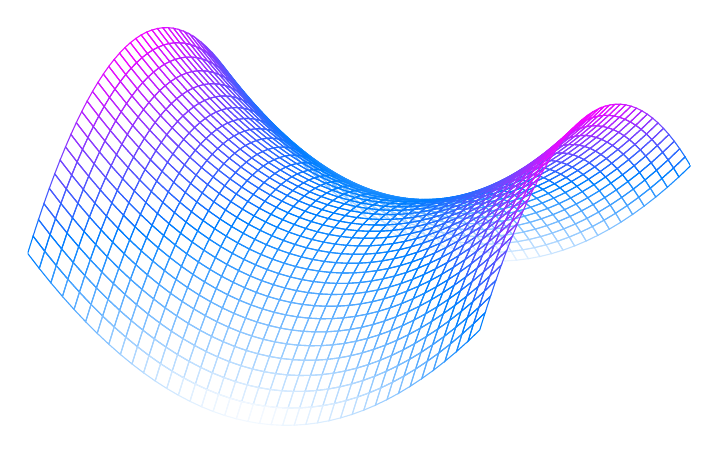
\begin{tikzpicture}\begin{axis}[hide axis,
xlabel=$x$,ylabel=$y$,colormap/cool, ]
\addplot3[domain=-3:3,mesh,samples=40]{x^2-y^2};
\end{axis}\end{tikzpicture}\end{center}
\newpage
\tableofcontents
\newpage

\section{Limits} \subfile{revisedsections/IntroToLimits}\newpage
\subsection{Types of Limits} \subfile{revisedsections/TypesOfLimits} \newpage
\subsection{Estimating Limits}
\subsection{The Squeeze Theorem}
\subsection{L'h\^{o}pital's Rule}
\subsection{Asymptotes}
\subsection{Relative Magnitudes}
\subsection{Continuity}

\section{Derivatives}
\subsection{Difference Quotient}
\subsection{Estimating Derivatives}
\subsection{Rules}
\subsection{Implicit Differentiation}
\subsection{Maxima \& Minima}
\subsection{Concavity}
\subsection{Graphical Relations}
\subsection{Relationship with Continuity}

\section{Applications of Derivatives}
\subsection{Units}
\subsection{Instantaneous Rate of Change}
\subsection{Tangent Line Approximations}
\subsection{Physics}
\subsection{Related Rates}
\subsection{Optimization}
\subsection{Differential Equations}
\subsection{Slope Fields}
\subsection{Mean Value Theorem}

\end{document}